% Figure F5_gain_vs_effort of study_analysis_001 - generated by thesis/study_analysis/figures.py; do not edit by hand.
% Preamble: \usepackage{pgfplots}
%           \pgfplotsset{compat=1.18}
% Net correctness gain vs repair output tokens
% Caption: figures/F5_gain_vs_effort.caption.tex (figure_caption_tex)
% Composite block; one point per (model, variant): repair output tokens of the variant's repair candidates vs net gain of Q06 correctness pass; descriptive only (no ranking, no test)
% Point labels (model): 1 = claude_fable_5; 2 = claude_opus_5; 3 = deepseek_v4_flash; 4 = deepseek_v4_pro; 5 = gemini_31_pro; 6 = gemini_36_flash; 7 = openai_gpt55; 8 = openai_gpt56_sol; 9 = qwen36_35b_a3b; 10 = qwen37_max; 11 = qwen3_coder_api
% BL01: Includes dense_la/00 (BL-01 tolerance convention: possible false FAIL verdicts; disclosure-bearing aggregate); sensitivity SA1 in T10.
% REASONING: Reasoning settings differ between models and are not equalised (see the closure disclosure register, item reasoning_policy_differences); some providers report no reasoning-token field.
% IC1: Q06 is in-sample for test_feedback and combined_feedback: their loops see the ParEval test verdict and stop when it passes (every stopped_tests_pass trajectory is a Q06 pass), so they optimise the endpoint; for static_feedback Q06 is out-of-sample (measured once in phase 2, never seen by the loop). The variants therefore differ in trigger and stop rules, not only in feedback content; test_feedback cannot regress on Q06 by construction.
% IC2: E02 is not an independent confirmation of Q06 gains: it counts build failures, and most E02 improvements are the same cells as the Q06 improvements; the held-out signal proper is the joint transition X06 (e.g. Q06 repaired but E02 still failing) and G01.
% IC6: static_feedback repair triggers are dominated by clang-tidy bugprone findings and, on MPI, by low-confidence hints (design document: no trustworthy static MPI tool exists); static_feedback results measure this frozen blocking-set configuration, not static analysis in general.
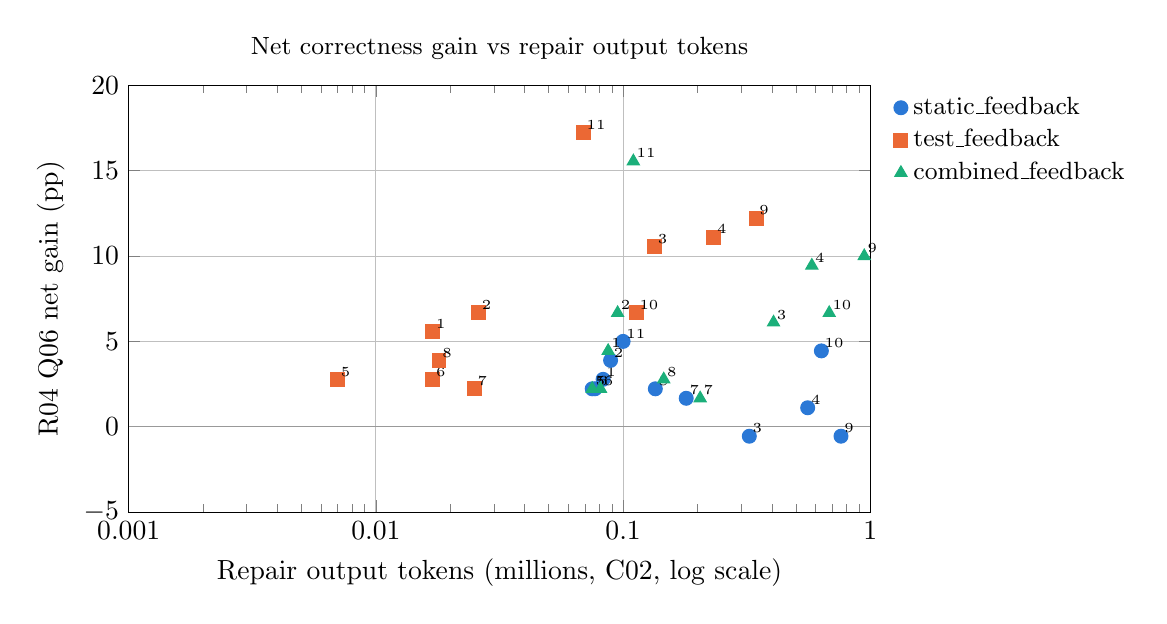
\begin{tikzpicture}
\definecolor{saSeriesA}{HTML}{2A78D6}
\definecolor{saSeriesB}{HTML}{EB6834}
\definecolor{saSeriesC}{HTML}{1BAF7A}
\begin{axis}[
  width=11cm,
  height=7cm,
  xmin=0.001,
  xmax=1.000,
  ymin=-5.000,
  ymax=20.000,
  xlabel={Repair output tokens (millions, C02, log scale)},
  ylabel={R04 Q06 net gain (pp)},
  grid=major,
  legend cell align=left,
  legend style={at={(1.02,1)},anchor=north west,font=\small,draw=none},
  xmode=log,
  log basis x=10,
  log ticks with fixed point,
  title={Net correctness gain vs repair output tokens},
  title style={font=\small}
]
\addplot[draw=black!40, forget plot] coordinates {(0.001,0) (1.000,0)};
\addplot[only marks, mark=*, color=saSeriesA, mark size=2.5pt, nodes near coords, point meta=explicit symbolic, every node near coord/.append style={font=\tiny, text=black, anchor=south west, inner sep=1pt}] coordinates {(0.083,2.778) [1] (0.089,3.889) [2] (0.324,-0.556) [3] (0.558,1.111) [4] (0.075,2.222) [5] (0.077,2.222) [6] (0.180,1.667) [7] (0.135,2.222) [8] (0.761,-0.556) [9] (0.634,4.444) [10] (0.100,5.000) [11]};
\addlegendentry{static\_feedback}
\addplot[only marks, mark=square*, color=saSeriesB, mark size=2.5pt, nodes near coords, point meta=explicit symbolic, every node near coord/.append style={font=\tiny, text=black, anchor=south west, inner sep=1pt}] coordinates {(0.017,5.556) [1] (0.026,6.667) [2] (0.134,10.556) [3] (0.233,11.111) [4] (0.007,2.778) [5] (0.017,2.778) [6] (0.025,2.222) [7] (0.018,3.889) [8] (0.345,12.222) [9] (0.113,6.667) [10] (0.069,17.222) [11]};
\addlegendentry{test\_feedback}
\addplot[only marks, mark=triangle*, color=saSeriesC, mark size=2.5pt, nodes near coords, point meta=explicit symbolic, every node near coord/.append style={font=\tiny, text=black, anchor=south west, inner sep=1pt}] coordinates {(0.087,4.444) [1] (0.095,6.667) [2] (0.406,6.111) [3] (0.580,9.444) [4] (0.075,2.222) [5] (0.081,2.222) [6] (0.205,1.667) [7] (0.146,2.778) [8] (0.945,10.000) [9] (0.682,6.667) [10] (0.110,15.556) [11]};
\addlegendentry{combined\_feedback}
\end{axis}
\end{tikzpicture}
